\begin{enumerate}
\item What value should we get if we sum all of the
angles that appear around one of the interior vertices in the 
finished diagram?  Verify that all three have the correct sum.

\begin{center}
\begin{picture}(0,0)%
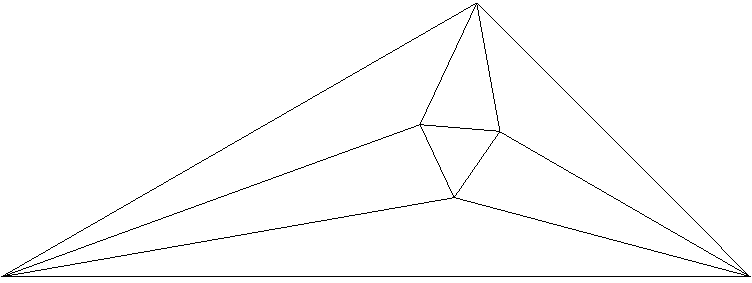
\includegraphics{figures/Morley_finished.pdf}%
\end{picture}%
\setlength{\unitlength}{3947sp}%
%
\begingroup\makeatletter\ifx\SetFigFont\undefined%
\gdef\SetFigFont#1#2#3#4#5{%
  \reset@font\fontsize{#1}{#2pt}%
  \fontfamily{#3}\fontseries{#4}\fontshape{#5}%
  \selectfont}%
\fi\endgroup%
\begin{picture}(6013,2252)(1191,-3877)
\put(1877,-3530){\makebox(0,0)[lb]{\smash{{\SetFigFont{12}{14.4}{\familydefault}{\mddefault}{\updefault}{\color[rgb]{0,0,0}$a$}%
}}}}
\put(2009,-3808){\makebox(0,0)[lb]{\smash{{\SetFigFont{12}{14.4}{\familydefault}{\mddefault}{\updefault}{\color[rgb]{0,0,0}$a$}%
}}}}
\put(1942,-3654){\makebox(0,0)[lb]{\smash{{\SetFigFont{12}{14.4}{\familydefault}{\mddefault}{\updefault}{\color[rgb]{0,0,0}$a$}%
}}}}
\put(4595,-3190){\makebox(0,0)[lb]{\smash{{\SetFigFont{12}{14.4}{\familydefault}{\mddefault}{\updefault}{\color[rgb]{0,0,0}$b^{\star}$}%
}}}}
\put(4392,-2806){\makebox(0,0)[lb]{\smash{{\SetFigFont{12}{14.4}{\familydefault}{\mddefault}{\updefault}{\color[rgb]{0,0,0}$c^{\star}$}%
}}}}
\put(4253,-2611){\makebox(0,0)[lb]{\smash{{\SetFigFont{12}{14.4}{\familydefault}{\mddefault}{\updefault}{\color[rgb]{0,0,0}$b^{\star\star}$}%
}}}}
\put(4723,-1915){\makebox(0,0)[lb]{\smash{{\SetFigFont{12}{14.4}{\familydefault}{\mddefault}{\updefault}{\color[rgb]{0,0,0}$c$}%
}}}}
\put(5094,-1936){\makebox(0,0)[lb]{\smash{{\SetFigFont{12}{14.4}{\familydefault}{\mddefault}{\updefault}{\color[rgb]{0,0,0}$c$}%
}}}}
\put(4919,-1942){\makebox(0,0)[lb]{\smash{{\SetFigFont{12}{14.4}{\familydefault}{\mddefault}{\updefault}{\color[rgb]{0,0,0}$c$}%
}}}}
\put(4683,-3383){\makebox(0,0)[lb]{\smash{{\SetFigFont{12}{14.4}{\familydefault}{\mddefault}{\updefault}{\color[rgb]{0,0,0}$c^{\star\star}$}%
}}}}
\put(6478,-3804){\makebox(0,0)[lb]{\smash{{\SetFigFont{12}{14.4}{\familydefault}{\mddefault}{\updefault}{\color[rgb]{0,0,0}$b$}%
}}}}
\put(6509,-3633){\makebox(0,0)[lb]{\smash{{\SetFigFont{12}{14.4}{\familydefault}{\mddefault}{\updefault}{\color[rgb]{0,0,0}$b$}%
}}}}
\put(6570,-3475){\makebox(0,0)[lb]{\smash{{\SetFigFont{12}{14.4}{\familydefault}{\mddefault}{\updefault}{\color[rgb]{0,0,0}$b$}%
}}}}
\put(4610,-2604){\makebox(0,0)[lb]{\smash{{\SetFigFont{12}{14.4}{\familydefault}{\mddefault}{\updefault}{\color[rgb]{0,0,0}$a^{\star}$}%
}}}}
\put(4986,-2628){\makebox(0,0)[lb]{\smash{{\SetFigFont{12}{14.4}{\familydefault}{\mddefault}{\updefault}{\color[rgb]{0,0,0}$b^{\star}$}%
}}}}
\put(5221,-2672){\makebox(0,0)[lb]{\smash{{\SetFigFont{12}{14.4}{\familydefault}{\mddefault}{\updefault}{\color[rgb]{0,0,0}$a^{\star\star}$}%
}}}}
\put(5135,-2863){\makebox(0,0)[lb]{\smash{{\SetFigFont{12}{14.4}{\familydefault}{\mddefault}{\updefault}{\color[rgb]{0,0,0}$c^{\star}$}%
}}}}
\put(4902,-3203){\makebox(0,0)[lb]{\smash{{\SetFigFont{12}{14.4}{\familydefault}{\mddefault}{\updefault}{\color[rgb]{0,0,0}$a^{\star}$}%
}}}}
\end{picture}%

\end{center}

\item In this section we talked about similarity.  Two figures in 
the plane are 
similar if it is possible to turn one into the other
by a sequence of mappings: a translation, a rotation and a scaling.  

Geometric similarity is an equivalence relation.  To fix our
notation, let $T(x,y)$ represent a generic translation, $R(x,y)$ a rotation
and $S(x,y)$ a scaling -- thus a generic similarity is a function from
$\Reals^2$ to $\Reals^2$ that can be written in the form $S(R(T(x,y)))$.

Discuss the three properties of an equivalence relation (reflexivity, symmetry and transitivity) in terms of geometric similarity.

\end{enumerate}

%% Emacs customization
%% 
%% Local Variables: ***
%% TeX-master: "GIAM-hw.tex" ***
%% comment-column:0 ***
%% comment-start: "%% "  ***
%% comment-end:"***" ***
%% End: ***

